\documentclass[11pt, a4paper, oneside, article]{memoir}
% Load the preamble
\usepackage{myproposal}

% Abbreviation glossary
\usepackage[acronym,nogroupskip,nonumberlist,toc]{glossaries}
\setglossarystyle{index}
\makeglossaries                         % Generate the glossary

% Bibliography with biblatex
\usepackage[style=authoryear-comp, bibstyle=authortitle, citestyle=authoryear-comp, maxcitenames=1, maxbibnames=100, sorting=nty, uniquelist=false, giveninits=true, backend=biber]{biblatex}
\addbibresource[location=local, datatype=bibtex]{atmo.bib}

\graphicspath{{pictures/}}              % Set graphics path

%DOCUMENT%
\begin{document}
\setlength{\baselineskip}{15pt}         % 15-20 pt

\input{latex_setup/abbreviations}

%\frontmatter
%\titlepage
\begin{center}
   \vspace*{-1\baselineskip}
    \huge
    \textbf{Lise Meitner Proposal}\\
    \vspace{0.5\baselineskip}
    \LARGE   
    \gls{odina}
    \vspace{0.5\baselineskip}
    \glsresetall
    \normalsize
    \tableofcontents*
\end{center}

\mainmatter
\chapter{Research context}
\label{c:context}
\begin{wrapfigure}[]{R}[0pt]{0.68\textwidth}
  % R - floating; r - h! [narrow lines] <- reduce whitespace below [17]
  \centering
  \includegraphics[width=0.66\textwidth]{evolution_of_climate_models}
  \caption{A growth and evolution timeline of climate models. The complexity of global climate models has increased enormously over the last four decades. The most powerful models, such as the \gls{cesm}, now have the capability of simulating a broad range of atmospheric processes, such as the impact of marine ecosystems on the atmosphere. \copyright \gls{ncar}.}
  \label{fig:growth_esm}
\end{wrapfigure}

\glspl{esm} have been rapidly evolving over the past decades (Fig.~\ref{fig:growth_esm}) thanks to growing computing power. But this development comes at the cost of a complexity rivaling the real world and immense resources for computing. To predict the response of the Earth’s ecosystem in a changing climate and its feedback on the very same climate, it is important to replace past parameterizations with our state-of-the-art understanding of the underlying processes. From solving the Navier-Stokes equations of wind and waves several decades ago, ESMs came to represent even biotical process of soil microbial and fungi. But the more we learn the more do we know what is left unknown. There are missing links and knowledge gaps especially when it comes to the details of the complex interaction between terrestrial ecosystems and the atmosphere. First analyses of \gls{cmip}~6 indicate a growing divergence between models, in particular in the land and atmospheric components. Although this will not revoke climate change, it still affects the reliability of model predictions.

\begin{wrapfigure}[]{R}[0pt]{0.5\textwidth}
  % R - floating; r - h! [narrow lines] <- reduce whitespace below [17]
  \centering
  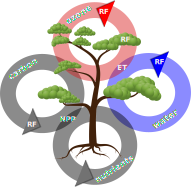
\includegraphics[width=0.48\textwidth]{ozone_es_scheme}
  \caption{Schematic view of the importance of ozone in \glspl{esm}. Ozone inflicts damage to vegetation. Ozone affects photosynthesis negatively and hence \gls{npp} ($\rightarrow$ carbon cycle). Ozone affects opening and closing of stomata (positively and negatively) and hence \gls{et} of plants ($\rightarrow$ water cycle). Both affect the processing of nutrients ($\rightarrow$ nutrient cycle). Ozone damage on vegetation causes positive and negative feedback on tropospheric ozone concentrations and hence on air quality and \gls{rf} \parencite{Nat:Sitch2007}.}
  \label{fig:ozone_esm_scheme}
\end{wrapfigure}

Ozone is an important trace gas in the atmosphere. In accordance with its effects and realm of occurence, we can distinguish the good (stratosphere), the bad (troposphere), and the ugly (ambient air) ozone. Here we shall focus on the connection and feedback between the bad and the ugly sides of ozone. Ozone is ranked third amongst the most potent climate forcers. It contributes to warming in the troposphere where it is produced as a secondary air pollutant in chemical cycles involving precursors such as CO and NOx as well as hydrocarbons (VOC, BVOC). Ozone is highly toxic and harmful to human health and many ecosystems. Despite a successful reduction of precursors in recent years leading to a stagnation of the upward trend in tropospheric ozone concentrations, there are indications that climate feedback on the ozone uptake by land biosphere can hamper reaching the ultimate air quality goal \parencite{NCC:Lin2020}. In drought conditions, plants will limit their transpiration by closing their stomata, which regulate all gas exchange of the plant, while emitting BVOCs at the same time and thus increase surface ozone concentrations. Ozone uptake through plants’ stomata is considered one of the most effective removal pathways of ozone, which will lead to a double penalty of climate change on vegetation and air quality. But large uncertainties in non-stomatal removal remain \parencite{RG:Clifton2020}.
Besides air quality consideration, ozone interferes with the climate and Earth system both directly and indirectly. Directly ozone affects the radiative forcing through its absorbance in both long and short wave bands and hence our assessment on climate change. In this project I will focus on indirect feedback on climate and air quality through ozone impact on vegetation. A high cumulative uptake of ozone (CUO) leads to considerably visible (e.g. necrosis, early senescence) and invisible damage (e.g. reduced photosynthesis) on vegetation (enter citations here). Ozone damage reduces plant photosynthesis and stomatal conductance and therefore interferes directly with net primary production (NPP) and (evapo)transpiration (ET) (Fig.~\ref{fig:schema_ozone_esm}). As depicted in Fig.~\ref{fig:schema_ozone_esm}, ozone uptake by vegetation and consequent damage, interfere with several sensitive parts of the Earth system. Ozone stress affects net primary production (NPP) and gross primary production (GPP) and hence CO2 removal from the atmosphere. Which has consequences on the nutrient cycle. At the same time, physical damage will alter evapotranspiration (ET) of the plant. Depending on the species and severity of damage both a reduced or an increased have been reported \parencite{SR:Hoshika2015}. 
Accounting for ozone induced reduction of stomatal conductance and photosynthesisI independently, \textcite{BGS:Lombardozzi2012} could improve model predictions of GPP and transpiration on global scales. \textcite{BGSD:Franz2020} show potential ozone damage on vegetation under climate change scenarios involving explicit modeling on the plant physiological level. These previous studies have not included an online atmospheric chemistry with known caveats. 
Empirically it was found that ozone damage leads to a reduced maximum electron transport rate $\mathrm{J_{max}}$ and maximum carboxylation efficiency Vcmax \parencite{EJA:Emberson2018} which are the basic processes involved in photosynthesis. Because the ratio $\mathrm{J_{max}}$:Vcmax is found to be constant (even under ozone exposure), the main traits of ozone induced damage can be modeled by a relative reduction in $\mathrm{J_{max}}$ alone (Falk et al., 2021 in preparation)\parencites{BGS:Franz2017}{BGS:Franz2018}.
Here, we want to combine the efforts of process understanding at the vegetation level into a fully coupled ESM with atmospheric chemistry and state-of-the-art nutrient limited carbon sequestration and study the feedback of ozone damage and thermal stress on air quality targets and climate.





\chapter{Aims \& hypothesis}
\label{c:aim_hyp}
The project \gls{odina} focuses on the process-based modelling of ozone induced damage on vegetation. To this end the applicant will implement a two-way coupling of ozone between the atmosphere and land-biosphere in the widely used global climate model \gls{cesm}. \gls{odina} studies the vegetations' feedback on near-surface to tropospheric ozone concentrations and will improve our understanding on the process-level. The improved capabilities of \gls{cesm} including the \gls{odina} model will be demonstrated in future projection using the high emission \gls{ssp}~5 scenario to study \textbf{\color{red}ozone} concentrations in the light of air quality regulations. \gls{odina} will also enable the research team to study ozone impacts through vegetation on the global \textbf{\color{darkgray}carbon cycle} and \textbf{\color{blue}water cycle}, and thus ultimately climate.
The \gls{odina} project is guided by five \textbf{working hypotheses}: 

\begin{enumerate}
\itemsep0pt
\item Elevated ozone concentration levels affect plant physiology via reduced stomatal conductance and photosynthesis. 
\item Reduced stomatal conductance will decrease ozone uptake by vegetation and hence diminish the dry deposition sink of ozone to the land biosphere. This will in turn give  positive feedback and lead to higher ground-level ozone concentrations in regions with damaged vegetation, and thus degrade ambient air quality.
\item Decreasing stomatal conductance will further affect transpiration of plants implicating lower relative humidity and less cooling by latent heat. At the same time more water will remain in the soil.
\item A reduction of photosynthesis will affect the carbon sequestration, the terrestrial carbon sink, and hence diminish the removal of \ch{CO_2} from the atmosphere.
\item All described feedback mechanisms may increase surface air temperature and thus amplify local/regional temperature extremes.
\end{enumerate}

Guided by these hypotheses, the project team will specifically
\begin{enumerate}
\itemsep0pt
\item Investigate the interaction between ozone and plant physiology and quantify on the one had the degree of plant damage to be expected through elevated ozone levels and on the other the expected increase in ozone burden due to reduced dry deposition.
\item Quantify the effect of plan health on \gls{bvoc} emissions and subsequent effects on ozone air quality.  
\item Quantify the effect of reduced stomatal conductance and thus photosynthesis on carbon sequestration and thus climate forcing.
\end{enumerate}



\chapter{Innovation}
\label{c:innovation}
Although \textbf{\color{red}ozone damage} has been addressed previously as reviewed in Section~\ref{sec:review}, ozone damage has not been included on the process level into a nutrient cost driven photosynthesis and at the same time coupled to both atmosphere and atmospheric chemistry, in \gls{cesm}.

Such extension of the \gls{cesm} model is a timely effort given the importance of the process and the extensive model user base. The \gls{cesm} user community extends worldwide, with about $4,000$ registered users in the support forum, and its importance for scientific discovery is reflected in about $3,000$ research and development papers published since 2009.

\important{Without doubt, new developments in such a widely used model will have a lasting impact on the climate and air quality research communities. Besides the advancement of our modelling capacities the proposed research will contribute to a more complete understanding of surface air quality, and more robust future projections, and represent an improvement beyond the capabilities reflected in \gls{cmip}~5 or \gls{cmip}~6 generation models.}


\chapter{Research methods \& model description}
\label{c:methods}
The research will apply and extend the latest release series of the \gls{cesm} and its components, \gls{clm}~5 including \gls{bvoc} emissions (\gls{megan} model \parencite{ACP:Guenther2006}, \gls{cam}~6 with online (super-fast) chemistry (\gls{impact} model, \textcite{JGR:Rotman2004}). Below, we provide  a brief technical account of the model components of \gls{cesm} most relevant to the planned work, \gls{clm} including \gls{megan}, and \gls{cam}. Subsequently we review  the Lombardozzi model of ozone damage and close by introducing the new process oriented plant physiological model of ozone damage, developed by the applicant, including the planned integration into \gls{clm} that stands at the core of the \gls{odina} project.

\begin{wrapfigure}[33]{R}[0pt]{0.5\textwidth}
  % R - floating; r - h! [narrow lines] <- reduce whitespace below [17]
  \centering
  \includegraphics[width=0.48\textwidth]{ozone_luna_scheme}
  \caption{Schematic view of \gls{odina} model integration into \gls{clm}~5. Round boxes represent affected tropospheric chemistry (\gls{cam}-chem) and trace gas concentrations, e.g. \ch{[CO_2]}, \ch{[O_3]}, \ch{[H_2O]}. Annotated arrows denote associated process. Squared boxes represent processes in the land model (\gls{clm}). Plants \textbf{\color{darkgray}invest carbon} to \textbf{\color{darkgray}take up nutrients}. A variable \ch{C:N} ratio at leaf level steers the optimization of electron transport ($\mathrm{J_{max}}$) and carboxylation rate ($\mathrm{V_{cmax}}$), which determine photosynthesis ($\mathrm{A_n}$) and stomatal conductance ($\mathrm{g_{sto}}$). $\mathrm{g_{sto}}$ controls transpiration and thus \textbf{\color{blue}plant hydraulics}. \textbf{\color{red}Ozone uptake} is determined by $\mathrm{g_{sto}}$ and reduces both $\mathrm{J_{max}}$ and $\mathrm{V_{cmax}}$.
}
  \label{fig:ozone_odina}
\end{wrapfigure}

\section{Community Earth System Model (CESM)}
\label{sec:cesm}
In \gls{clm}~5, \textbf{photosynthesis} (and hence the {\color{darkgray}carbon cycle}) is tied to \textbf{\color{darkgray}plant nutrient dynamics} (dark gray boxes in Fig.~\ref{fig:ozone_odina}) which incorporates the \textbf{\gls{fun}} model \parencites{GBC:Fisher2010}{JGR:Brzostek2014}{GCB:Shi2015}. The concept of \gls{fun} is that nitrogen uptake requires an investment of energy (e.g. carbon) and that there is a large number of potential sources of nitrogen available in the environment. The ratio of carbon invested to acquire nitrogen is therefore treated as a cost in the model. \gls{fun} calculates the rate of symbiotic nitrogen fixation for nitrogen that is passed directly to the plant, and subsequently delivered and incorporated  as inorganic ammonium in the soil \parencite{GBC:Cleveland1999}, separately. Nutrient limitation is represented by a variable plant \ch{C:N} ratio which allows plants to adjust their \ch{C:N} ratio at the leaf level at the cost of nitrogen \parencite{JAMES:Ghimire2016}. The \textbf{\gls{luna}} model \parencites{STE:Xu2019}{GMD:Ali2016} finally links these processes with photosynthesis. To this end the \gls{luna} model calculates the photosynthetic capacity based on optimization of the use of leaf nitrogen under different environmental conditions. \textbf{Stomatal conductance} is based on this \textbf{nitrogen-limited photosynthesis} rather than on potential photosynthesis. The maximum stomatal conductance is obtained from the \textbf{Medlyn stomatal conductance} model \parencite{GCB:Medlyn2011} which is preferred over Ball-Berry-type models \parencite{BallBerry1987} for it’s more realistic behavior at low humidity levels (high vapor pressure deficit) \parencites{PR:Rogers2013}{NP:Rogers2017}.

As a \textbf{plant hydraulic stress} routine explicitly models water transport through the vegetation according to a simple hydraulic framework \parencite{JAMES:Kennedy2019}, stomatal conductance is also a function of prognostic leaf water potential and hence forced by transpiration. Plant water stress is calculated as the ratio of attenuated stomatal conductance to maximum stomatal conductance.

\textbf{Biogenic emissions} from vegetation are not directly integrated into the modelling framework described above but handled by \gls{megan} \parencite{ACP:Guenther2006}. \gls{megan} uses above canopy atmospheric forcing, e.g. solar radiation, temperature, and moisture, and \ch{[CO_2]} as input variables. \gls{megan} receives only \gls{lai} as vegetation input information, which can be either prescribed (\gls{sp} mode) or dynamic (\gls{bgc} mode) and \gls{pft}. In \gls{clm}~5, \gls{megan}~version~2.1 \parencite{GMD:Guenther2012} is implemented. \gls{megan}~2.1 includes 147 chemical compounds which can be subset and grouped together (e.g. \emph{isoprene} = pentane + hexane + heptane + tricyclene). In \gls{clm}, trapping of emissions inside of the canopy is explicitly disabled (i.e., escape efficiency set to 1).

In \textbf{\gls{cam}-chem}, \textbf{dry deposition} follows the resistance approach originally described by \textcites{AE:Wesely1989}{AE:Walcek1986} and updated sequentially \parencites{AE:Walmsley1996}{AE:Wesely2000}. All deposited chemical species are mapped to a weighted-combination of ozone and sulfur dioxide depositions to characterize their oxidation potential versus their solubility in water which is dependent on the effective Henry’s law coefficient of the species. All species in the mechanism are per default affected by dry deposition if deposition velocities are defined. The computation of \textbf{deposition velocities} (or resistances) ties \gls{cam}-chem to \gls{clm}. Dry deposition velocities vary with \gls{pft}. A grid-averaged velocity is computed as the weighted-mean over all land cover types. The impact from changes in land cover, land use or climate are thus directly reflected in the coupled model \parencite{GMD:Lamarque2012}. 

\section{Ozone damage in CESM}
\label{sec:ozone_damage}
\textbf{At present, ozone damage on vegetation is not reliably accounted for in \gls{cesm}}. There are a couple of technical reasons for this. First of all, the land surface model (\gls{clm}) as a stand-alone model would need at least a reliable global climatology to integrate ozone damage in its default setup. Global ozone reanalysis (i.e. \gls{cam} reanalysis products of \gls{ecmwf}) or satellite derived tropospheric ozone would be candidates but show, despite improvements in recent years, considerable biases compared to observations \textbf{\color{blue}Added: \parencites{GMD:Huijnen2020}{ACPD:Barten2020}}. Though ozone climatologies based on older \gls{cesm} runs with \gls{cam} and \gls{clm} exist \parencite{ACP:Lamarque2010}, common caveat of such simulations with uncoupled ozone are
\begin{enumerate}
\itemsep0pt
\item inconsistency between the land surface (e.g. land use type, roughness length) used in the \gls{ccm} and the uncoupled land surfaces model with ozone damage functions, and
\item ozone concentrations are not provided to \gls{clm} directly from the atmosphere and therefore mostly not in agreement with atmospheric abundances.
\end{enumerate}

\textbf{Ozone damage in \gls{clm}~5} is based on the work of Lombardozzi \textcite{Oe:Lombardozzi2012} which showed an effective decoupling of $A_\mathrm{n}$ and $g_\mathrm{sto}$ under high \gls{cuo}, with $g_\mathrm{sto}$ being less sensitive to cumulative uptake of ozone. If taken into consideration this improves global projections of \gls{gpp} and transpiration considerably \parencite{BGS:Lombardozzi2012}, especially in tropical regions as also shown by \textcite{Nat:Sitch2007} and \textcite{ACP:Pacifico2015}. In this implementation, damage coefficients for $g_\mathrm{sto}$ and $A_\mathrm{n}$ are defined for coniferous, deciduous, and non-woody \glspl{pft}, respectively. \gls{cuo} can be regulated through an uptake threshold $\Phi_\mathrm{th}$, further a healing factor is computed based on change in \gls{lai} (growth of new leaves). \textbf{\color{blue}Added text: Technical limitations and issues of the current ozone damage module include its disconnection from the nutrient and carbon cost driven photosynthesis and compatibility with the plant hydraulic module. In particular, the order in which stomatal conductance is reduced under combined thermal and oxidative stress is not clearly constrained.} 

\textbf{\color{blue}Added text:Recent model development efforts led by the applicant have addressed some of the limitations listed above by integrating ozone damage on the process-level. A linear linear relationship between \gls{cuo} and $\mathrm{J_{max}}$ in forced and control experiments was deduced based on the body of peer reviewed research articles published in recent years.} The \gls{odina} model integrates seamlessly into existing, scientifically validated modules in \gls{clm} (e.g. \gls{fun}, \gls{luna}). The integration of \gls{odina} into the existing framework of \gls{clm}~5 is schematically illustrated in Fig.~\ref{fig:ozone_odina}. \gls{odina} also builds on previous efforts by \textcites{BGS:Lombardozzi2012}{Oe:Lombardozzi2012}, leading to a comprehensive database of experimental data of ozone damage and an implementation of an ozone damage module in \gls{clm}~4 \parencite{BGS:Lombardozzi2013}. This database will be used for model evaluation of \gls{odina} as data are not included in the derivation of the linear relationship detailed above. One of the advantages of the \gls{odina} model is that it can be used to study ozone effects on the \ch{C:N} ratio and thus \textbf{\color{red}TODO: Add meaning if C:N ratio for plants}.

\important{The purpose of this project is to establish the coupling of \gls{clm}~5 to \gls{cam}-chem with respect to ozone through dry deposition and evaluate the comprehensive two-way coupling of ozone-vegetation in the light of progressing climate change.}


\chapter{Intended collaborations}
\label{c:collab}

The applicant will collaborate within the \gls{odina} project also closely with core developers of \gls{cesm} at the \gls{ncar/ucar} in Boulder, \acrshort{col}, \acrshort{usa}. Tasks in \gls{wp}~2 (see Chapter~\ref{c:project_plan}) will be partially performed during a research stay at \gls{ncar/ucar} hosted by Dr.~Louisa Emmons (Atmospheric Chemistry Observations \& Modeling Lab) and Dr.~Dave Lawrence (Climate \& Global Dynamics Lab) and their teams, see letter of collaboration in \hyperref[fig:loi_ncar]{Annex~5}. 
In particular, the applicant will benefit from technical support by the core developers of the \gls{cesm} concerning the code integration and coupling of atmospheric \ch{[O_3]} to \gls{odina} described in \glspl{wp}~1--2 (Section~\ref{sec:wp1}--\ref{sec:wp2}). Furthermore, the offered guidance by the \gls{ncar/ucar} community, in particular by the land-modeling and atmospheric groups during the planed research stay, will foster valuable connections and experience for future career perspectives.
The \gls{odina} project will benefit from the established contacts with \gls{ncar/ucar} also in the later phase \glspl{wp}~3--4 (Section~\ref{sec:wp3}--\ref{sec:wp4}) with respect to analysis and assessment of the modeling results. Both sides are expected to benefit from the contributions by the applicant and \gls{boku} to future development of the \gls{cesm}.

Additional collaboration will include the technical and scientific staff at the \gls{uio} (Norway), particularly Prof. Terje K. Berntsen (Section for Meteorology and Oceanography) and the \gls{clm} Norway team (see letter of collaboration in \hyperref[fig:loi_uio]{Annex~5}). 
The mountainous landscapes of both Austria and Norway pose similar challenges for \gls{esm} modeling, wherefore both sides will benefit from continuing existing collaborations within the \gls{emerald} project during \gls{odina}. The future involvement of the applicant and \gls{boku} in \gls{cesm} development will also benefit its sister~model the \gls{noresm}, and thereby modeling initiatives of the Norwegian partners.
Furthermore, it is planned to utilize the potential of the land-modelling platform developed at \gls{uio} in collaboration with the applicant during her stay for the purpose of site-level model evaluation in \gls{wp}3 (Section~\ref{sec:wp3}). 

\chapter{Work plan \& timeline}
\label{c:project_plan}
As specified in the call for the Lise-Meitner Fellowship the project plan is aligned for a duration of 24~months. The project is divided into five tangible \glspl{wp} of varying duration (Fig.~\ref{fig:flowchart}). \gls{wp}0 (Management and mentoring) and \gls{wp}5 (Reporting and dissemination) are designed to run through the whole project duration of 24~months concomitantly (Fig.~\ref{fig:ganttchart}).

\gls{wp}0 oversees the whole project and is central for the career development guided by the host institution. \gls{wp}0 has also a bi-directional component as mentoring and support is received by the applicant as well as given through co-supervision of master and PhD students. All communication, e.g. regular reporting to the \gls{fwf} and dissemination in the form of research papers, conference contributions, and public outreach activities, are bundled in \gls{wp}5. The scientific and technical work is assigned to \glspl{wp}~1--4. The technicality of the \glspl{wp} is decreasing from \gls{wp}1 (mainly technical) to \gls{wp}4 (purely scientific) with expected increasing scientific throughput. \gls{wp}1 (Model integration) and \gls{wp}2 (Model coupling) are tightly interlinked with \gls{wp}3 (Model evaluation) spanning the whole duration of \gls{wp}1 and \gls{wp}2. \gls{wp}2 depends on the realisation of \gls{wp}1, and \gls{wp}4 depends on the completion of all previous substantial \glspl{wp}~1--3. Each \gls{wp} has companion \glspl{ms} assigned. Further details on these \gls{ms} are presented in Section~\ref{sec:milestones}.\\

\begin{figure}[!ht]
  \centering
  %\subbottom[Flow chart]{%
    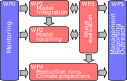
\includegraphics[width=0.75\textwidth]{wp_flow_chart}
    \caption{Flow chart of the \gls{odina} project, with \glspl{wp} as presented in this Section. All \glspl{wp} are embedded in \gls{wp}0 which coordinates the subordinate \glspl{wp}. \gls{wp}1 and \gls{wp}2 comprise the most technical aspects: integration of the \gls{odina} model into the \gls{clm}, coupling of \gls{odina} to the \gls{cam}-chem, and improvement of the dry deposition scheme. \gls{wp}2 is accompanied by a research stay at the \gls{ncar/ucar} lab in Boulder, \acrshort{col}, \acrshort{usa}. The \gls{wp}3 focuses on the evaluation of the \gls{odina} model performance. \gls{wp}4 comprises the production and analysis of long-term simulations (\gls{cmip}~6 style) and their comparison to available \gls{cesm} baseline simulations. \gls{wp}5 communicates an reports results continuously.}
  \label{fig:flowchart}%}\\
  \vspace{-1\baselineskip}
\end{figure}

Prof.~Rieder and members of his research group will support Dr.~Falk in all scientific, technical, and administrative matters of the \gls{odina} project. Individual contributions of the team members to \gls{odina} are specified below.\\

Prof.~Rieder will act as mentor to Dr.~Falk within \gls{odina}. He will devote 10\% of his time as in-kind support distributed across all \glspl{wp}. He will provide guidance on all scientific aspects of the project, the dissemination of results to scientific and lay audiences, and the advising and mentoring of students (PhD and MSc). Most importantly however, he will provide career counseling and support Dr.~Falk in growing her professional network, international, nationally and at the host institution, as well as assist her in developing and refining her leadership philosophy. Prof.~Rieder will also provide guidance regarding the selection of different trainings for staff development offered by \gls{boku} and make recommendations for additional courses or workshops offered by scientific unions or third-party providers. Further details on the mentor-mentee relationship are detailed in the career development plan in \hyperref[appendix:career]{Annex 3}.

Dr.~Alexander will support Dr.~Falk in all matters related to scientific computing. He will assist in model porting, model architecture and \gls{hpc} on the \gls{vsc} and in-house \gls{hpc} infrastructure. He will devote 10\% of his time as an in-kind contribution to \gls{odina}, distributed on \glspl{wp}~1,~2,~and~4. 

Dr.~Mayer will support Dr.~Falk in \glspl{wp}~1, 3, 4, and 5. Particularly, she will contribute to model evaluation and analyses tailored to quantify effects of two-way coupled ozone dry deposition on ambient air quality and plant health. She will devote 10\% of her time as an in-kind contribution to \gls{odina} and act as mentor to Dr.~Falk.    

Mr.~Staehle, Msc, is a PhD student in the Rieder group focusing on the climate-air quality-health nexus. His research is supported by institutional funds of \gls{boku}. He will contribute 50\% of his time as in-kind support to the \gls{odina} project, particularly \glspl{wp}~3--5. He will be jointly supervised on this research by Dr.~Falk and Prof.~Rieder.

Mrs.~Hasenhündl and Mrs.~Falmbigl are the administrative assistants of the host institute. They will support Dr.~Falk in all administrative matters during the course of the \gls{odina} project as well as during the preparation and the relocation phase upon receipt of the funding notice.\\

The host institute will provide all infrastructure necessary for a seamless implementation of the \gls{odina} project. This includes access to the national \gls{hpc} resources at \gls{vsc}, including private nodes and state-of-the-art storage and post-processing servers in-house at \gls{boku}. Upon approval of the \gls{odina} project Prof.~Rieder and Dr.~Alexander will assist Dr.~Falk in an application to obtain additional core hours on \gls{vsc} for \gls{odina}, which are commonly granted on basis of the operator agreement regarding peer-reviewed projects that require large computational resources. \gls{boku} will provide further office space, desktop \acrshort{it} equipment, and access to libraries and other university facilities. 

\vspace{-0.5\baselineskip}
\section{WP0 Management \& mentoring}
\label{sec:wp0}
The management and mentoring \gls{wp}, spans the entire project period and includes a variety of bi-directional tasks in cooperation and with support of the faculty host and host institute at \gls{boku}. \gls{wp}0 is built upon the core attributes of the Lise-Meitner Fellowship and shall enable the applicant to position herself as an emerging leader in land-atmosphere interactions, particularly the climate-vegetation-air quality nexus. During the start phase of the \gls{odina} project, \gls{wp}0 will ensure a smooth integration into the work environment at the host institute and involves all aspects concerning technical, administrative and logistic support by the corresponding units of \gls{boku} (\ref{itm:start}). The mid-phase is split into the development and honing of key skills for a future leadership role in Earth science (\ref{itm:career_dev}) and monitoring of the project progress (\ref{itm:progress}). \ref{itm:career_dev} includes leadership and management training but also programs focusing on didactic skills, presentation techniques, public outreach formats, as well as co-supervision of students. A detailed career development plan is presented in \hyperref[appendix:career]{Annex 3}. In the end-phase \gls{wp}0 will initiate the preparation of follow-up proposals tailored to European and national funding schemes such as e.g. the \gls{fwf} Elise Richter Program or Stand-Alone projects (\ref{itm:followup}).

\vspace{-0.5\baselineskip}
\subsection*{Work Package duration 24 months (months 1 to 24)}
\begin{enumerate}[start=1,label={T0.\arabic*}]
  \itemsep0pt
\item Setup and project start \hfill [month 1]\label{itm:start}
\item Career development \hfill [month 1 -- 24]\label{itm:career_dev}
\item Progress monitoring \hfill [month 1 -- 23]\label{itm:progress}
\item Follow-up projects \hfill [month 18 -- 24]\label{itm:followup}
\end{enumerate}

\vspace{-1\baselineskip}
\section{WP1 Model integration}
\label{sec:wp1}
The model integration \gls{wp} will build on existing collaborations with technical and scientific staff at the \gls{uio} (Norway) and at \gls{ncar/ucar} in Boulder (\acrshort{col}, \acrshort{usa}) and include support by the scientific and technical team of the host institute at \gls{boku}, Vienna. Existing parts of the \gls{odina} model will be extended to describe our process understanding as accurately as possible. This will comprise
\begin{enumerate}
  \itemsep0pt
\item to include a state of stomata sluggishness and take a more explicit healing formulation into consideration (\ref{itm:slugg}) and
\item to deduce and update additional model parameters based on existing databases (\ref{itm:para}).
\end{enumerate}
It is expected that the model output considering active ozone damage will substantially differ between the updated (this proposal) and current \gls{cesm} configuration (\gls{cmip}~6). Initial cross-evaluation with data at global scales (coarse resolution model integration) and single site simulations (\ref{itm:init_sim}) following the \gls{cesm} standard procedures are likely to reveal the necessity for adjustment of additional free model parameters. An in-depth evaluation of individual parameters and results is subject to \gls{wp}3.

\vspace{-0.5\baselineskip}
\subsection*{Work Package duration 4 months (months 1 to 4)}
\begin{enumerate}[start=1,label={T1.\arabic*}]
  \itemsep0pt
\item Implementation of stomatal sluggishness and healing \hfill [month 1 -- 2]\label{itm:slugg}
\item Deduction of additional parameters \hfill [month 2 -- 3]\label{itm:para}
\item Initial model simulations and cross-evaluation \hfill [month 3 -- 4]\label{itm:init_sim}
\end{enumerate}

\section{WP2 Model coupling}
\label{sec:wp2}
Activities related to model coupling will include an extended research stay at the \gls{ncar/ucar} lab in Boulder (\acrshort{col}, \acrshort{usa}) to both facilitate the technical work as well as build important networks for future research activities. A one-way coupling between the atmospheric chemistry component (e.g. \gls{cam}-chem) to the land-surface component (\gls{clm}) is achieved through the dry deposition implementation already in place in \gls{cesm}. The existing dry deposition scheme in \gls{cesm} will be evaluated concerning \gls{odina}. If necessary, the scheme will be improved and updated (\ref{itm:drydep}). Two-way coupling will be achieved by propagating instantaneous ozone concentrations from the atmosphere through the coupler to the land component (\ref{itm:couple}). Technically this involves touching the \gls{cesm} coupler infrastructure. The work on the coupling will be done in the most sustainable way during the planned research stay at \gls{ncar/ucar}. Potential infrastructure updates will be taken into consideration and integrated into the workflow. Initial tests and evaluation of the coupled model on coarse-grid global-scale as well as through single site simulations are planned (\ref{itm:couple_test}). Detailed evaluation of the coupled model performance will be pursued in coordination with \gls{wp}3.
{
\subsection*{Work package duration 5 months (months 4 to 8)}
\begin{enumerate}[start=1,label={T2.\arabic*}]
  \itemsep0pt
\item Evaluation of the dry deposition scheme (improvement and update) \hfill [month 4 -- 5]\label{itm:drydep}
\item Technically coupling \gls{cam}-chem ozone concentrations to \gls{odina} \\$\rightarrow$ research stay at \gls{ncar/ucar} \hfill [month 5 -- 6]\label{itm:couple}
\item Perform model tests of the coupling algorithm \hfill [month 6 -- 8]\label{itm:couple_test}
\end{enumerate}
}

\section{WP3 Model evaluation \& update of model parameters}
\label{sec:wp3}
The evaluation of the updated model is an integral part of \gls{wp}1 and \gls{wp}2 and spans the whole duration of both \glspl{wp}. Data for evaluation will be collected from Fluxnet sites with associated ground level ozone observations, e.g. the \gls{airbase} (\ref{itm:eval_data}). Based on the collected data, the initial integration and validation tests are complemented and completed with more in depth evaluation for the selected sites (\ref{itm:eval_site}) and on global scales (\ref{itm:eval_glob}). In conjunction with \ref{itm:eval_site} the project team will work closely with the \gls{clm} team Norway at \gls{uio}. This will utilize also the land-modelling platform developed in collaboration with the applicant during her PostDoc at \gls{uio}. Variable model parameters will be adapted and adjusted if necessary to further improve the resulting model skills in terms of, e.g. \gls{npp}/\gls{gpp} (\ref{itm:update_para}). A model development and evaluation paper is pursued in coordination with \gls{wp}5.
{
\subsection*{Work Package duration 11 months (months 1 to 11)}
\begin{enumerate}[start=1,label={T3.\arabic*}]
  \itemsep0pt
\item Collection of evaluation data \hfill [month 1 -- 3]\label{itm:eval_data}
\item Site level evaluation \hfill [month 3 -- 6]\label{itm:eval_site}
\item Global scale evaluation \hfill [month 6 -- 11]\label{itm:eval_glob}
\item Update model parameters \hfill [month 3 -- 11]\label{itm:update_para}
\end{enumerate}
}

\vspace{0.5\baselineskip}
\section{WP4 Production runs \& future projections}
\label{sec:wp4}
Upon successful implementation of \gls{wp}~1--3 work on \gls{wp}4 is initiated. Within this final research \gls{wp} production runs with climate projections will be performed. It is planned to perform at least one long-term \gls{cmip} style ($1850-2100$) coupled model simulation (\ref{itm:ssp5}). As the highest tropospheric ozone abundances are expected for a low mitigation scenario with high anthropogenic greenhouse gas emissions and simultaneous substantial methane release from permafrost regions \parencites[e.g.][]{JGR:Rieder2015}{AE:Rieder2018}, \gls{ssp}~5 is selected as a future scenario. Additional simulations following other \glspl{ssp} are planned but completion will depend on the workload of the \gls{vsc} and thus cannot be guaranteed to be fully achieved within the 24~month project timeline. Of special interest are implications on future surface ozone abundance and air quality indices (\ref{itm:eval_ozone}) along with induced plant damage and effects on the carbon cycle (\ref{itm:eval_clim}), e.g. expected reduction in \gls{gpp} with respect to reference simulations. The focus herein lies on populous and highly industrialized regions, e.g. Europe, East Asia, North America. To quantify the effects on carbon sequestration and climate, long-term simulations with the updated \gls{cesm} for comparison with existing \gls{cmip}~6 simulations will be conducted. Two scientific papers are expected to emerge out of \gls{wp}4, one focusing on future ozone air quality the other on ozone related plant damage.
{
\subsection*{Work Package duration 14 months (months 11 to 24)}
\begin{enumerate}[start=1,label={T4.\arabic*}]
  \itemsep0pt
\item Coupled \gls{cesm} simulation on climatological timescales (\gls{ssp}5) \hfill [month 11 -- 17]\label{itm:ssp5}
\item Evaluate climate and vegetation impacts on surface ozone abundance \hfill [month 11 -- 17]\label{itm:eval_ozone}
\item Quantify the effects on carbon sequestration and climate forcing. \hfill [month 17 -- 24]\label{itm:eval_clim}
\end{enumerate}
}

%\vspace{0.5\baselineskip}
\section{WP5 Reporting \& dissemination}
\label{sec:wp5}
\gls{wp}5 acts as an umbrella for reporting to the funding agency (\gls{fwf}) and dissemination to scientific and lay audiences. \gls{wp}5 spans the whole project duration and is effectively the coordinating and reporting hub for \gls{wp}1--4. Science communication (\ref{itm:communication}) is further divided into research papers, conference contributions, and public outreach. 
At least three research papers are expected to emerge out of the \gls{odina} project, one focusing on model development and evaluation, one on future changes in ambient air quality and one on ozone induced plant damage and effects on the carbon cycle.
Public outreach will include among others contributions to popular science blogs or presentations to the general public. Dissemination using social media platforms such as twitter will be considered if applicable. In close interaction with \gls{wp}0 and under guidance by the host institution, targeted networking activities are planned (e.g. conferences, workshops, professional networks) (\ref{itm:networking}). The submission of the final report to the funding agency (\gls{fwf}) is officially concluding \gls{wp}5 (\ref{itm:prep_reports}) although several additional papers are expected to emerge from the project past official completion.
{
\subsection*{Work Package duration 24 months (months 1 to 24)}
\begin{enumerate}[start=1,label={T5.\arabic*}]
  \itemsep0pt
\item Science communication \hfill [month 3 -- 24]\label{itm:communication}
\item Networking \hfill [month 1 -- 24]\label{itm:networking}
\item Prepare annual reports to funding agency (\gls{fwf}) \hfill [month 12 / 24]\label{itm:prep_reports}
\end{enumerate}
}

\vspace{0.5\baselineskip}
\section{Milestones}
\label{sec:milestones}
Each \gls{wp} has companion \glspl{ms} assigned. In Fig.~\ref{fig:ganttchart}, the colored bars represent the \glspl{wp} while the \glspl{ms} are denoted with a star. \gls{ms}0a marks the mid-term evaluation of the Lise-Meitner Fellowship program, while its completion is denoted by \gls{ms}0b. \gls{ms}1--3 mark the successful completion of \gls{wp}1--3, respectively. \gls{ms}4a marks the completion of the long-term \gls{cmip}~6 style simulations and is followed by the completion of the assessment and analysis of the model results (\gls{ms}4b) regarding impacts of the updated \gls{cesm} on air quality and climate. \gls{ms}5 comprises the annual reporting to the \gls{fwf} (2~reports).

\begin{enumerate}[start=0,label={MS\arabic*}]
  \itemsep0pt
  \item
  \begin{enumerate}[a]
  \item Mid-term evaluation of the career development and mentoring program \ \hfill [month 12]
  \item Completion of career development and mentoring program \hfill [month 24]
  \end{enumerate}
\item \quad Completion of model integration \hfill [month 4]
\item \quad Completion of model component coupling \hfill [month 8]
\item \quad Completion of initial model simulations and cross-evaluation \hfill [month 11]
\item 
\begin{enumerate}[a]
    \item Completion of model long-term \gls{cmip}~6 style simulations \hfill [month 17]
    \item Completion of analysis of \gls{cesm} long-term simulations \hfill [month 20]
\end{enumerate}
\item 
  \begin{enumerate}[a]
  \item Research article submission \hfill [month 13 / 22 / 24]
  \item Annual reports to funding agency (\gls{fwf}) \hfill [month 12 / 24]
  \end{enumerate}
\end{enumerate}

\begin{figure}[!ht]
  \centering
  %\subbottom[Gantt chart]
   %\vspace{-30pt}
\end{figure}



\chapter{Research-related qualifications of the researchers involved}
The applicant, \textbf{Stefanie Falk}, is a physicist by training. Her postdoctoral stations included the \gls{kit} and the \gls{uio}. Her curiosity about the complex and important role of ozone in the atmosphere led her from studying its chemical depletion in the stratosphere and polar boundary layer to its formation and removal processes by the land biosphere. Interdisciplinary work has been a cornerstone in her work to improve the understanding and push the development of current numerical models of the Earth system forward. In particular, she has been working on \gls{ccm} using the \gls{emac} model. Her work was related to future trends of stratospheric ozone, biogenic brominated \gls{vsls}, and the influence of sulfur aerosols. During her engagement at \gls{kit}, she also implemented a bromine release mechanism from snow and studied ozone depletion in the Arctic boundary layer. Identifying dry deposition as a key issue for both future air quality as well as climate, she committed to studies on the effects of ozone on vegetation in her latest work at \gls{uio}. From ozone formation and dry deposition on global and regional scales, her focus shifted later to process-based impact modeling at the leaf level and improvements of subarctic biomes. Her work resulted in scientific publications and conference contributions both nationally and internationally. She gladly participates in public outreach, at \gls{uio} through public lectures and popular science blogs in the Norwegian language. She is a member of the \gls{dpg} and the professional body of the environmental section in the \gls{dpg}, \gls{yess} community, and the \gls{eswn}.\\

\textbf{Harald Rieder} is full professor and head of the institute of meteorology and climatology at the University of Natural Resources and Life Sciences, Vienna. He is an expert in chemistry-climate connections. His research is centered on the climate-air quality-health nexus and combines numerical models with observational data sets from both ground-based networks and remote sensing platforms. He has led and extensively contributed to studies unravelling the effect of changes in climate, ambient meteorology, and anthropogenic emissions on surface pollution as well as the effects of atmospheric composition changes for climate at the surface and at upper atmospheric levels. Prof. Rieder serves among others as board member of the Austrian Centre for Climate Change and Member of the \gls{isac} Atmosphere Working Group.


\chapter{Ethical, safety-related, or regulatory aspects}
No other research of ethical, security-related or regulatory issues is foreseen. 


\chapter{Sex-specific \& gender-related issues}
The project does not raise any sex-specific and gender-related issues.


\chapter{Information on the research institution \& career development}
\label{c:info_dev}
\section{Added value to be expected from this collaboration}
The \gls{odina} project shows excellent fit with the research priorities of the host institution. The \gls{boku}, Vienna is an international leader in environmental sciences with research priorities comprising the preservation and development of the environment and quality of life, management of natural resources and the environment and safeguarding food and health. Prof. Rieder’s group at \gls{boku} focuses on chemistry-climate connections, particularly the effects of changes in atmospheric composition on climate and air quality across temporal and spatial scales. Within the framework of \gls{odina} Dr. Falk and the host group would be the first to develop a fully coupled ozone module within the \gls{cesm} and apply it to study impacts and feedback mechanisms for plant health and air quality. Given the diversity of research within the \gls{boku} community that focuses on plant physiology and plant health the model development and research activities within \gls{odina} will pave the road for manifold research endeavors ahead, and thereby create a lasting resource for \gls{boku} and the Austrian research landscape. Furthermore, the updated model version will increase the portfolio of contributions of the Rieder group to international activities within the framework of \gls{igac} activities such as \gls{toar}-2 and \gls{ccmi}-2.

\section{Importance of the project for the academic and research reputation of the applicant and her career development}
The \gls{odina} project will allow the applicant to pursue her research interests and spearhead the inclusion of coupled ozone chemistry in one of the widest used community earth system models. Thereby she will be able to position herself as an emerging leader in the field of coupled modeling with focus on land-atmosphere interactions, particularly the climate-vegetation-air quality nexus. Interaction through model development and application with the \gls{cesm} core team and \gls{igac} community will expand and strengthen her peer network. The scientific and technical support of the host group and broader \gls{boku} community will provide an ideal environment for project implementation. The mentoring and career development program accompanying this proposal will prepare Dr. Falk for an academic career ahead.

\section{Career Plan}
\label{sec:career}
In her research Dr. Falk strives to advance our understanding of causes and effects of changes in the chemical composition of the Earth’s atmosphere. To this end she applies state-of-the-art earth system models and contributes to their continuous development to improve the process level understanding and reduce uncertainties and biases in model projections. Dr. Falk aims to establish herself as an independent researcher with focus on the climate-air quality-health nexus and strives to achieve a permanent academic position either via a tenure-track faculty line or a senior scientist appointment. The proposed Lise-Meitner Fellowship is an important stepstone towards this goal.

The research framework of the fellowship project \gls{odina} allows Dr. Falk to follow her research interest and strengthen her scientific and technical portfolio to propel her career. Dr. Falk will spend her Lise-Meitner fellowship in Prof. Rieder’s group at the \gls{boku}, guaranteeing a stimulating research environment and ideal project support infrastructure. Prof. Rieder and his team focus on chemistry-climate connections, particularly ozone, and embedment in the \gls{boku} community will provide rich opportunities for interaction with research teams focusing on plant health and biosphere-atmosphere interaction. Including a module for coupled ozone chemistry between the atmosphere and land-surface components of \gls{cesm} Dr. Falk will provide an important extension to one of the widest used earth system models and provide rich opportunities for colleagues focusing on ambient air quality, ozone dry deposition and ozone plant damage and plant physiology. Given the broad impact of the model extension and opportunity to explore processes and feedbacks in the atmosphere-land system the \gls{odina} project will allow Dr. Falk to establish herself as an emerging leader in the field of land-atmosphere interaction.

The model development activities of \gls{odina} will link Dr. Falk with the core development team of the \gls{cesm} model at the \gls{ncar} in Boulder, CO, USA. The connection to \gls{ncar}'s Atmospheric Chemistry Observations \& Modeling Lab and Climate \& Global Dynamics Lab will be fostered through a 3-month research stay in the first year of the project. The \gls{odina} project will embed Dr. Falk also in the \gls{toar}-2 and \gls{ccmi}-2 activities of the \gls{igac} Project and thereby substantially expand her professional network.

Throughout the project the interaction between the Dr. Falk and Prof. Rieder will focus on all aspects related to the mentees career development and the overall progress of the research project. To this end they will meet for discussions on a weekly basis. These meetings will focus on the one hand on project status, opportunities or challenges emerging and scientific findings, on the other on recently published research highlights in the field, emerging funding and employment opportunities, as well as upcoming conferences or trainings. Prof. Rieder will provide dedicated support to Dr. Falk throughout the project. He will provide guidance and counseling in all scientific and professional aspects, introduce Dr. Falk to his network of peers and promote her as guest speaker for institute seminars and conferences. He will further provide guidance in the leverage of research results for high-profile publication formats and the effective dissemination of research outcomes via traditional media and online platforms. Besides Prof. Rieder, Dr. Falk will obtain mentoring by Dr. Mayer (\gls{boku}-Met) and other peers in the \gls{eswn}.

As an affiliate of \gls{boku} Dr. Falk will have access to a wide range of training and career development programs offered by the university. These include among others leadership training and didactic training as well as a variety of courses tailored to strengthen skills in project acquisition and project management and the preparation of application packages for tenure-track or staff scientist positions or the preparation of a habilitation thesis. Dr. Falk will be further assisted through \gls{boku}’s programs within the framework of the Postdoc Coaching Group and individual career coaching sessions. During her fellowship at \gls{boku} Dr. Falk will also gain experience in the mentoring and co-advising of undergraduate and graduate students within Prof. Rieder’s group and be supported in dissemination and outreach activities by the university media and public relations office.

To ensure continued funding after the end of the Liese-Meitner funding period Prof. Rieder and the \gls{boku} office for research support, innovation \& technology transfer will support Dr. Falk in the development of applications to national and European Union research programs. Furthermore to ensure further collaboration Prof. Rieder and his team will and include Dr. Falk in their own applications submitted to these funding schemes.


%\vspace*{5cm}
\vfill
\vspace{5cm}

\begin{minipage}{.4\textwidth}

  \vspace{-43.5px}
  \includegraphics{pictures/sign_sf}

  \hrulefill
  
  \hspace*{0mm}\phantom{}Dr. Stefanie Falk
  
  \hspace*{0mm}\phantom{}Applicant
\end{minipage}%
\hfill
\begin{minipage}{.4\textwidth}

  \hrulefill
  
  \hspace*{0mm}\phantom{}Prof. Harald Rieder
  
  \hspace*{0mm}\phantom{}Co-Applicant
\end{minipage}




%Print the glossary
\printglossary[type=\acronymtype,title={List of abbreviations}]
%\printglossaries

\newpage

\backmatter
\setcounter{page}{1}
\appendix
\printbibliography[env=bibliography, title=Annex 1 - References]
\chapter{Annex 2 - CVs and description of previous research achievements}
\chapter{Annex 3 - Career plan}
\chapter{Annex 4 - Co-applicant's letter of recommendation}
\chapter{Annex 5 - Collaboration letters}
\chapter{Annex 6 - Additional recommendation}

\end{document}
